\section{Anonymity}
ein heuristisches Prinzip (Arbeitshypothese, vorläufige Annahme als Hilfsmittel der Forschung, Untersuchung, Erklärung)
\subsection{HEURISTIC 1}
If two (or more) addresses are inputs to the same transaction, they are controlled by the same user; i.e., for any transaction t, all pk $\in$ inputs(t) are controlled by the same user.\\
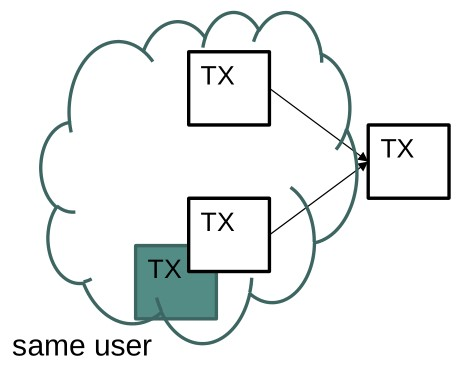
\includegraphics[width=\linewidth]{heuristic-1.jpg}

\subsection{HEURISTIC 2}
The one-time change address is controlled by the same user as the input addresses; i.e., for any transaction t, the controller of inputs(t) also controls the one-time change address pk $\in$ outputs(t) (if  such an address exists).\\
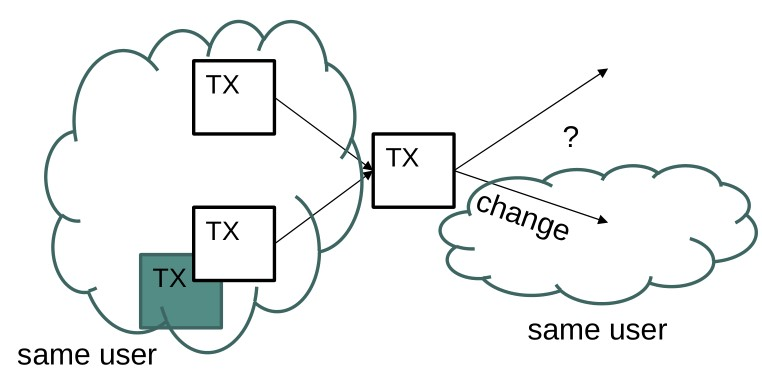
\includegraphics[width=\linewidth]{heuristic-2.jpg}

\subsection{HEURISTIC 3}
Multisig wallets usually use p2sh change, but the recipient rarely uses p2sh, which allows to determine the correct change output with high probability.\\
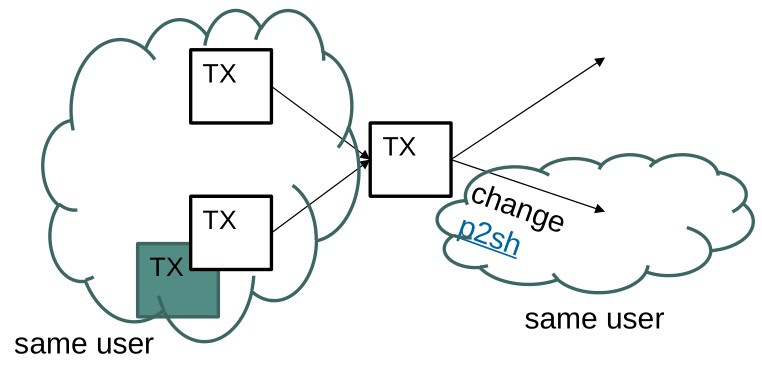
\includegraphics[width=\linewidth]{heuristic-3.jpg}

\subsection{OPTIMAL CHANGE HEURISTIC}
The assumption is that wallet software does not spend outputs unnecessarily. Therefore the change value is smaller than any of the spent outputs. Because if the change was larger than one output then this output would be left out and the change would be reduced by the output's value.\\
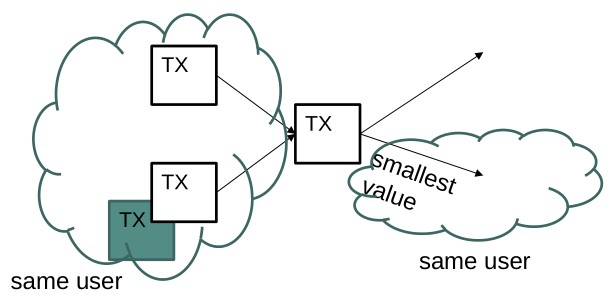
\includegraphics[width=\linewidth]{optimal-change-heuristic.jpg}

\subsection{CONSUMER HEURISTIC}
Consumer wallets only create transactions with two outputs. Therefore, if an output is spent by a transaction with 3 outputs it is not change.\\
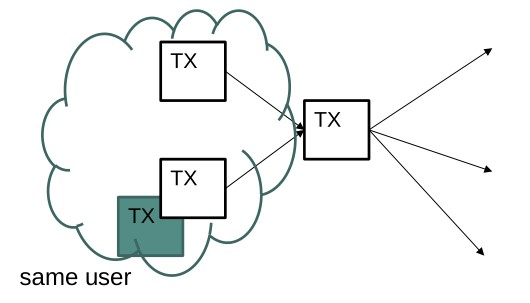
\includegraphics[width=\linewidth]{consumer-heuristic.jpg}

\subsection{Monero}
\begin{itemize}
  \item Confidential Block explorer (No Output or receiver)
  \item No scripting (no smart contracts)
  \item Proof of work algorithm (CPU Mining)
  \item Due to cryptographic algorithms, unknown: addresses trading monero,   amounts, address balances, or transaction histories.
  \item Malware mining, due to CPU bound Proof of Work
\end{itemize}